\documentclass[12pt]{book}
\usepackage{graphicx}
\usepackage{subfig} % make it possible to include more than one captioned figure/table in a single float
\usepackage[utf8]{inputenc}
\usepackage{hyperref}
\usepackage[intlimits]{amsmath}
\usepackage{amssymb}
\usepackage{tkz-euclide}
\usepackage{tikz}
\setlength{\oddsidemargin}{15.5pt} 
\setlength{\evensidemargin}{15.5pt}
\pretolerance=2000
\tolerance=3000
\renewcommand{\figurename}{Figura}
\renewcommand{\chaptername}{Cap\'{i}tulo}
\renewcommand{\contentsname}{\'{I}ndice}
\renewcommand{\tablename}{Tabla}
\renewcommand{\bibname}{Bibliograf\'{i}a}
\renewcommand{\appendixname}{Ap\'endices}


\title{Sistema autogravitante con simetría esférica y distribución exponencial de masa}
\date{}
\begin{document}
\section*{Nociones teóricas}

Para una distribución de masa $\rho$

\begin{description}
\item De la ley de Newton la fuerza gravitatoria ejercitada en el punto x es:  $F(x) = G \int{\frac{x\prime - x}{|x\prime - x|^3}\rho(x\prime)d^3x} $ y despues de hacer cálculos llegamos a $ \nabla F(x) = -4\pi G \rho(x) $
\item Definimos el potencial gravitatorio $\Phi(x) = -G \int{\frac{\rho(x\prime)}{|x\prime - x|}d^3x} $. Observamos que $F(x) = - \nabla \Phi $ y después de reemplazar en la ecuación de antes se obtiene la ecuación de Poisson: $\nabla^2 \Phi = 4\pi G \rho $
\item \textbf{En coordenadas esféricas} ($r,\theta,\varphi$) \textbf{con simetria esférica} 
(las funciones solo dependen de r y no de la posición en la esfera de radio r: los angulos $\theta$ y $\varphi$), asi que las derivadas totales coinciden con las derivadas parciales $\frac {d\Phi(r)}{dr} = \frac{\partial \Phi(r)}{\partial r} $; 
$\nabla \Phi(r) = \frac{\partial \Phi(r)}{\partial r} $ y 
$\nabla^2 \Phi(r) = \frac{1}{r^2} \frac{\partial }{\partial r}(r^2 \frac{\partial \phi(r)}{\partial r})$
La ecuacion Poisson:$ \frac{1}{r^2} \frac{\partial }{\partial r}(r^2 \frac{\partial \phi(r)}{\partial r}) = 4\pi G \rho(r) \implies
r^2 \frac{\partial \phi(r)}{\partial r} = 4\pi G \int{r^2\rho(r)dr} + K_1 \implies
\frac{\partial \Phi(r)}{\partial r} = \frac{4 \pi G}{r^2}\int{r^2\rho(r)dr} + \frac{K_1}{r^2}\implies
\Phi(r) = 4\pi G \int{\frac{1}{r^2}(\int{r^2\rho(r)dr})dr } + K_1\int{\frac{1}{r^2}dr} + K_2
=4\pi G \int{\frac{1}{r^2}(\int{r^2\rho(r)dr})dr } + \frac{K_1}{r} + K_2, K_1, K_2 \in \mathbb{R} (el signo - con K_1)
 $
\item Definimos la velocidad circular: la velocidad de una particula en una orbita circular de radio r:
$v_c^2(r) = r\frac{\partial \Phi(r)}{\partial r} \implies
v_c^2(r) = \frac{4\pi G}{r}\int{r^2\rho(r)dr} + \frac{K}{r}, K \in \mathbb{R} \implies 
v_c(r) = (\frac{4 \pi G}{r}\int{r^2\rho(r)dr} + \frac{K}{r})^{\frac{1}{2}}, K \in \mathbb{R}
$
\item La masa $M(r) = 4 \pi \int{r^2\rho(r)dr} + K, K \in \mathbb{R}$
\item En un sistema con simetria esférica: la proyección de una función f(r) en el plano y,z (a lo largo de la línea de visión OX)es la funcción: 
$F(s) = \int_{-\infty}^\infty{f(r)dx}$

$x^2 = r^2 - s^2 \implies dx = \frac{r dr}{\sqrt{r^2 - s^2}} \implies$
$F(s) =  2\int_s^\infty{\frac{r f(r)}{\sqrt{r^2-s^2}}dr}, s^2=y^2 + z^2$(s es el radio proyectado) (\url{http://en.wikipedia.org/wiki/Abel\_transform})
\item La proyección de la distribución de densidad en el plano Y0Z $D_p(s) =  2\int_s^\infty{\frac{r \rho(r)}{\sqrt{r^2-s^2}}dr}$,$s^2 = y^2 + z^2$ 

\begin{tikzpicture}[scale=.8]

% definitions
\tkzDefPoint(0,0){O}
\tkzDefPoint(2,2){P}
\tkzDefPoint(0,2){M}
\tkzDefPoint(3.5,0){Q}
\tkzDefPoint(2.87,2){S}
\tkzDefPoint(-2.87,2){T}


\tkzDrawCircle(O,Q)
\draw [shorten >= -5cm, shorten <=-5cm] (S)--(T) ;
\tkzDrawSegments[thick](O,M)
\tkzDrawSegments[thick](O,P)
\tkzDrawPoints(O,P,Q,T,M,S)

\node at (6,2.2){line of sight};
\node at (-0.5,1){s};
\node at (0.7,0.5){r};
\node at (0.5,2.2){x};
% labels
\tkzLabelPoints(Q,T,O,M,S,P)
\end{tikzpicture}
\end{description}

\section*{Problema de la práctica}
\begin{description}
\item Hipótesis: $\rho(r) = Ae^{-Br} = rhoC \dot e^{-\frac{r}{r_0}}, A,B > 0, rhoC = A, r_0=frac{1}{B}$  en un sistema con simetria esférica
\item Determinar $\Phi(r)$, M(r),$M_p(r)$, $v_c(r)$ 

\end{description}


\begin{description}
\item $\Phi(r) = 4 \pi G A \int{ \frac{1}{r^2}(\int{a^2 e^{-Ba}da})dr} + \frac{K_1}{r} + K_2$



\item Para poder calcular las integrales de forma numérica establecemos los límites de integración y cogemos los constantes 0
Miramos el gráfico de la función: f(r) = rhoC * exp(-r/r0)
\begin{figure}[!ht]
 \centering
 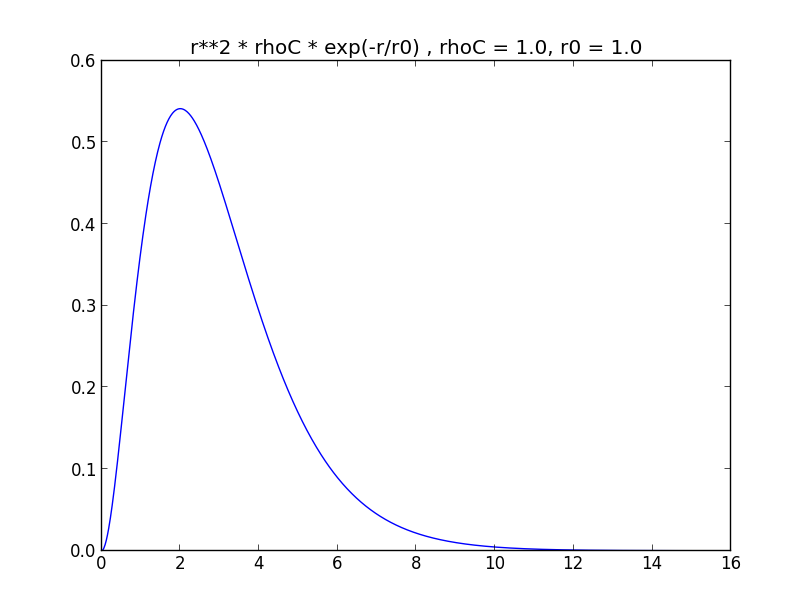
\includegraphics[scale=0.33]{func1Plot.png}
 \caption{\emph{rhoC * exp(-r/r0)}}
\end{figure}
observamos que  f es  continua y f(0) = 0
\item  $\int{r^2 e^{-Br}dr} = \int_0^r{x^2 e^{-Bx}dx}$


\item Integrando por partes 2 veces:
\item $\int_0^r{x^2 e^{-Bx}dx} = - \frac{1}{B} \int_0^r{x^2 (e^{-Bx})\prime dx}
=-\frac{1}{B}( (x^2 e^{-Bx})\Big|_0^r  - 2\int_0^r{x e^{-Bx}dx})  = -\frac{2}{B^2}\int_0^r{x (e^{-Bx})\prime dx} - \frac{1}{B}r^2 e^{-Br} = -\frac{2}{B^2}((x e^{-Bx})\Big|_0^r - \int_0^r{e^{-Bx}dx}) - \frac{1}{B}r^2 e^{-Br} = -\frac{2}{B^3}e^{-Bx}\Big|_0^r -\frac{2}{B^2}r e^{-Br} - \frac{1}{B}r^2 e^{-Br} = \frac{2}{B^3} -\frac{2}{B^3}e^{-Br} -\frac{2}{B^2}r e^{-Br} - \frac{1}{B}r^2 e^{-Br}  $
\item Miramos el gráfico de la función $f(r) = \frac{1}{r^2}  \int_0^r{\rho_c  e^{-\frac{r}{r0}}}$
que no está definida en 0 pero es continua en (0,$\infty$) y $  \lim_{x \underset{>}{\to} 0} f(x) = 0$
\begin{figure}[!ht]
 \centering
 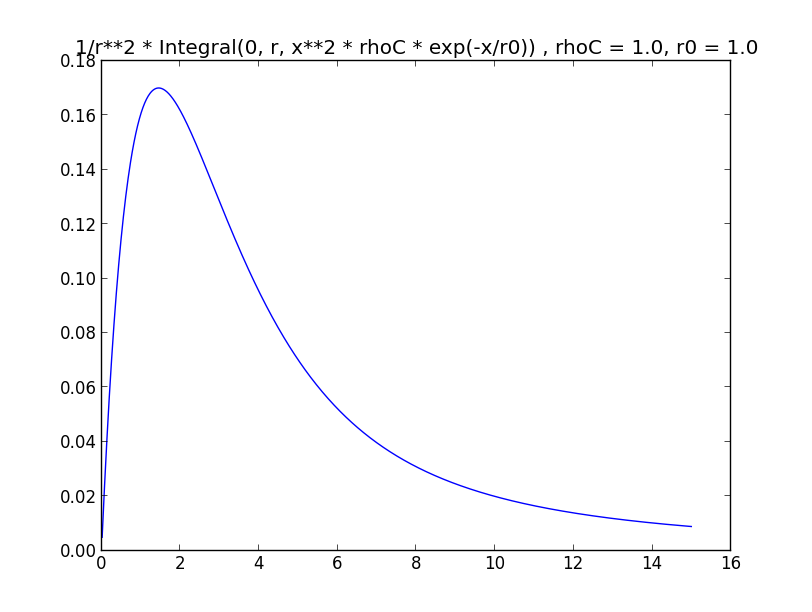
\includegraphics[scale=0.33]{func2Plot.png}
 \caption{\emph{rhoC * exp(-r/r0)}}
\end{figure}



\item $\implies \int_\varepsilon^r{ \frac{1}{x^2}(\int_0^x{y^2 e^{-By}dy})dx} = 
-\frac{1}{B}(-\frac{2}{B^2}\int_\varepsilon^r{\frac{1}{x^2}dx} +\frac{1}{B^2}\int_\varepsilon^r{\frac{1}{x^2}e^{-Bx}dx}  + \frac{2}{B}\int_\varepsilon^r{\frac{1}{x} e^{-Bx}dx} + \int_\varepsilon^r{e^{-Bx}dx} ) = 
\frac{1}{B^2}(\frac{2}{B}(\frac{1}{\varepsilon} - \frac{1}{r})  + e^{-Br} - \frac{1}{B}\int_\varepsilon^r{\frac{1}{x^2}e^{-Bx}dx} - 2\int_\varepsilon^r{\frac{1}{x} e^{-Bx}dx} ) $

\item $\implies \Phi(r) = \frac{4 \pi G A}{B^2}(\frac{2}{B}(\frac{1}{\varepsilon} - \frac{1}{r}) + e^{-Br} - \frac{1}{B}\int_\varepsilon^r{\frac{1}{x^2}e^{-Bx}dx} - 2\int_\varepsilon^r{\frac{1}{x} e^{-Bx}dx} ) $


\item $M(r) = 4 \pi A \int_0^r{x^2 e^{-Bx}dx} = -\frac{4 \pi A}{B}(\frac{2}{B^2} + \frac{2}{B^2}e^{-Br} +\frac{2}{B}r e^{-Br} + r^2 e^{-Br}) $
\item La proyección de la distribución de densidad en el plano YOZ
$D_p(s) = 2 A \int_s^\infty{\frac{r}{\sqrt{r^2-s^2}} e^{-Br} dr}$

\item $v_c(r) = (\frac{4 \pi G A}{r}\int_0^r{x^2 e^{-Bx}dx} )^{\frac{1}{2}}   
= (-\frac{4 \pi G A}{B}(\frac{2}{B^2r}e^{-Br} +\frac{2}{B} e^{-Br} + r e^{-Br} -  \frac{2}{B^2r} ))^{\frac{1}{2}} $

\end{description}


\begin{description}
\item Los gráficos se realizaron con un programa python (en el repositorio git: \url{https://github.com/beevageeva/potencial} ) tomando las constantes de integración 0 y usando las expresiones iniciales(sin hacer la integración por partes). 
Las integraciones se calculan de forma numérica y observando los gráficos de las funciones que se integran estas son continuas y tienen el valor 0 en el punto 0 así que se pueden tomar los límites de integración 0 y r.
Se muestran los gráficos para la función de densidad $ rhoC * e^{\frac{-r}{r_0} }$ variando rhoC y $r_0$ con valores 0.5, 1 y 2


\item

\begin{figure}[!ht]
 \centering
 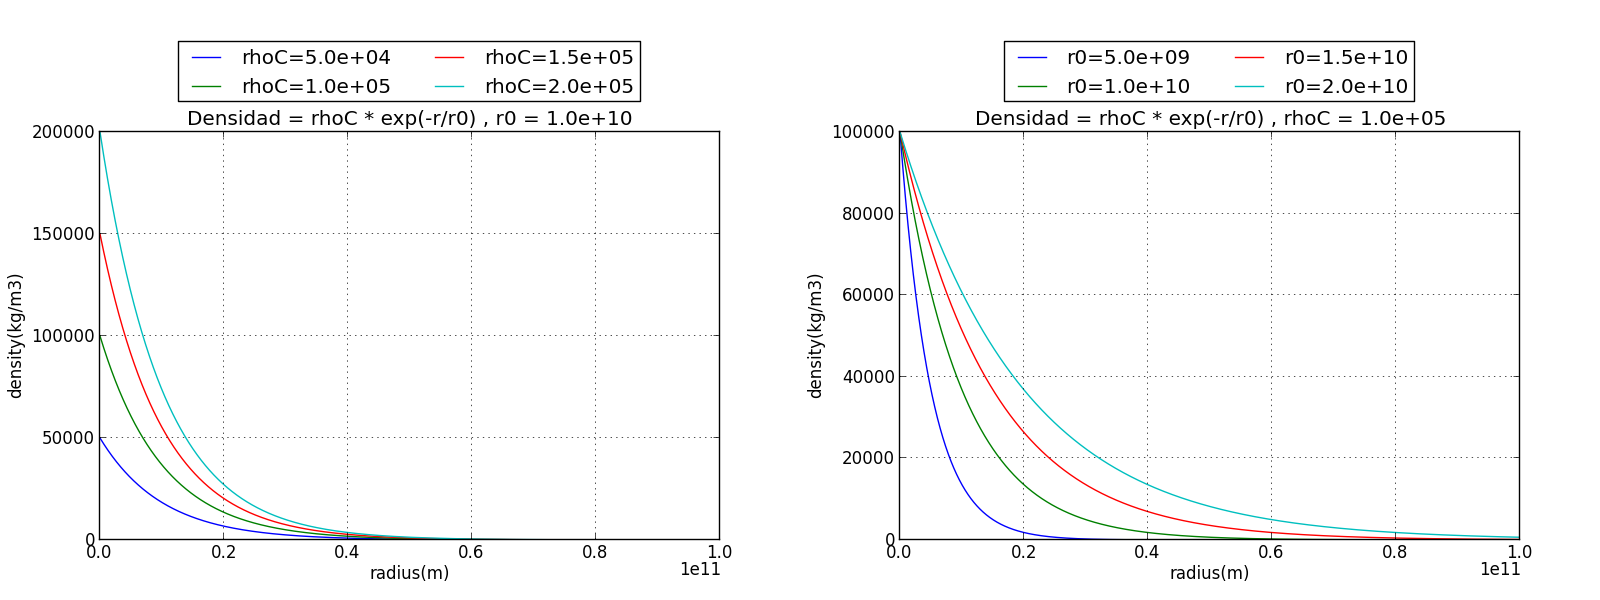
\includegraphics[scale=0.33]{densFinal.png}
 \caption{\emph{Densidad}}
\end{figure}

\item

\begin{figure}[!ht]
 \centering
 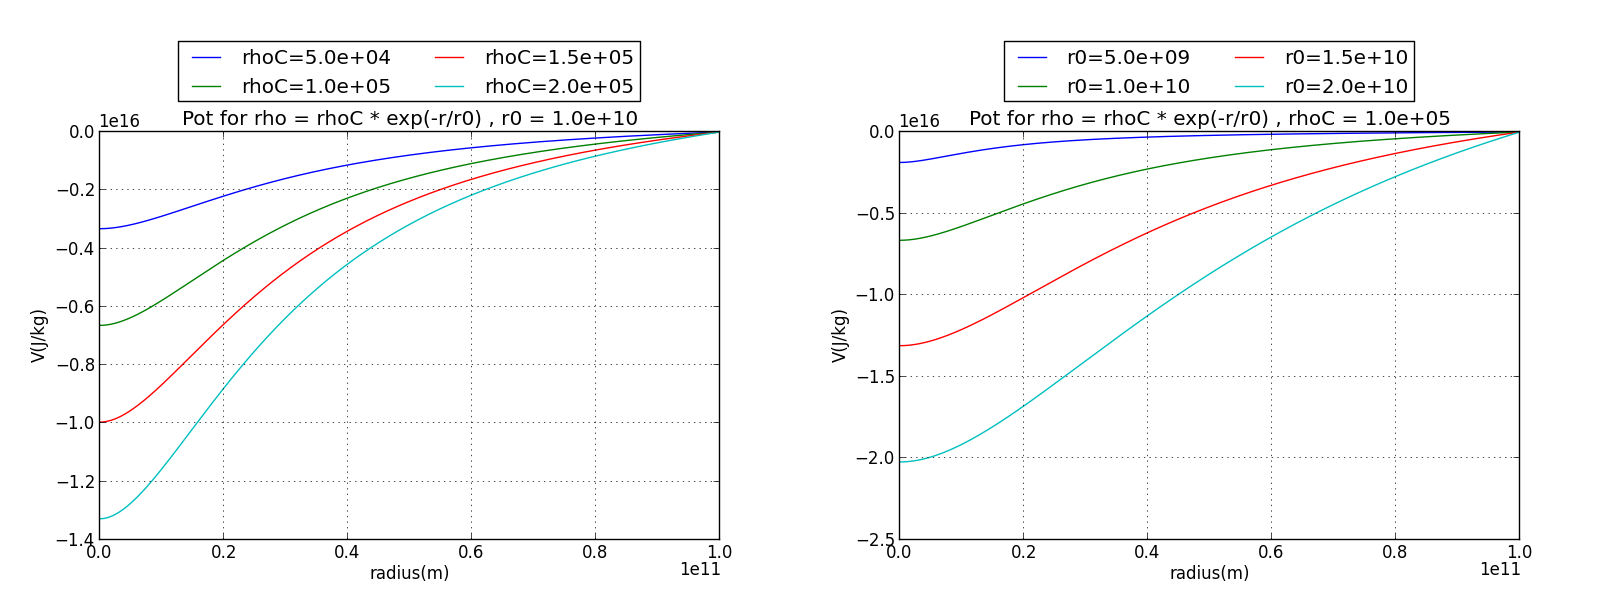
\includegraphics[scale=0.33]{potFinal.png}
 \caption{\emph{Potencial}}
\end{figure}

\item

\begin{figure}[!ht]
 \centering
 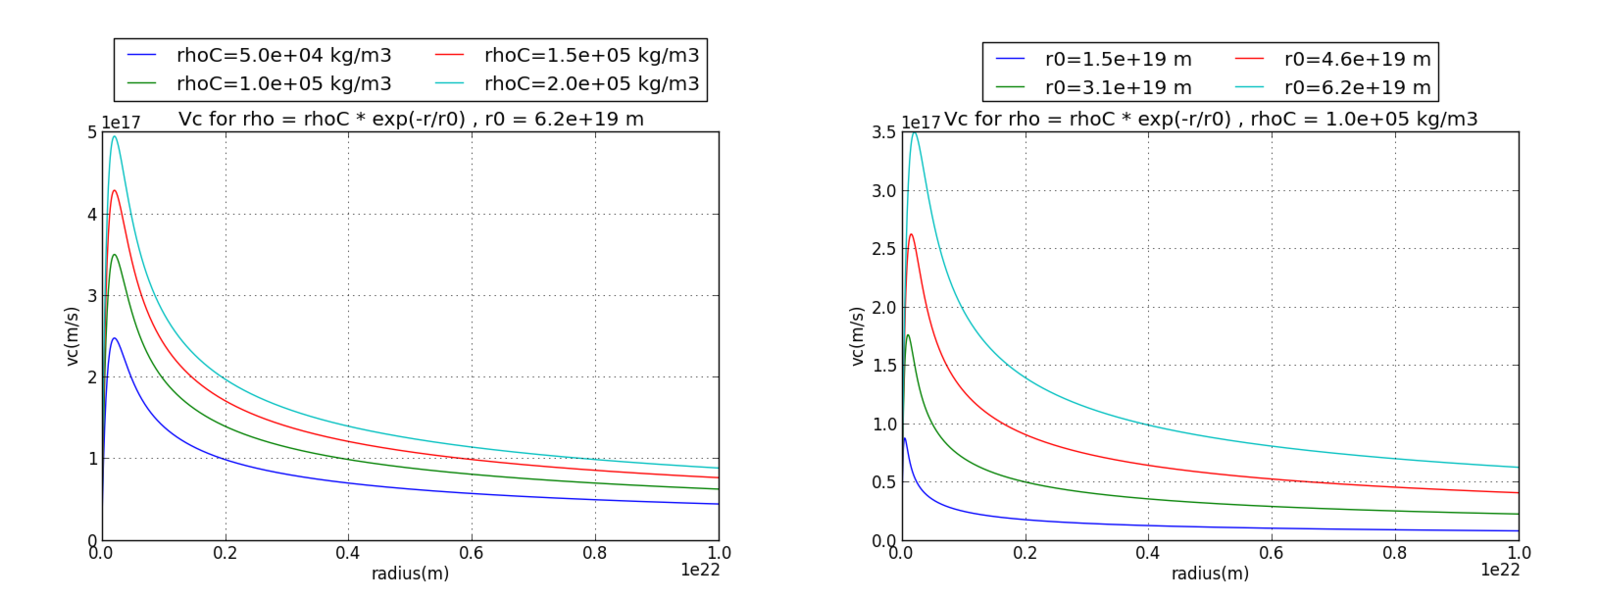
\includegraphics[scale=0.33]{vcFinal.png}
 \caption{\emph{Velocidad circular}}
\end{figure}

\item

\begin{figure}[!ht]
 \centering
 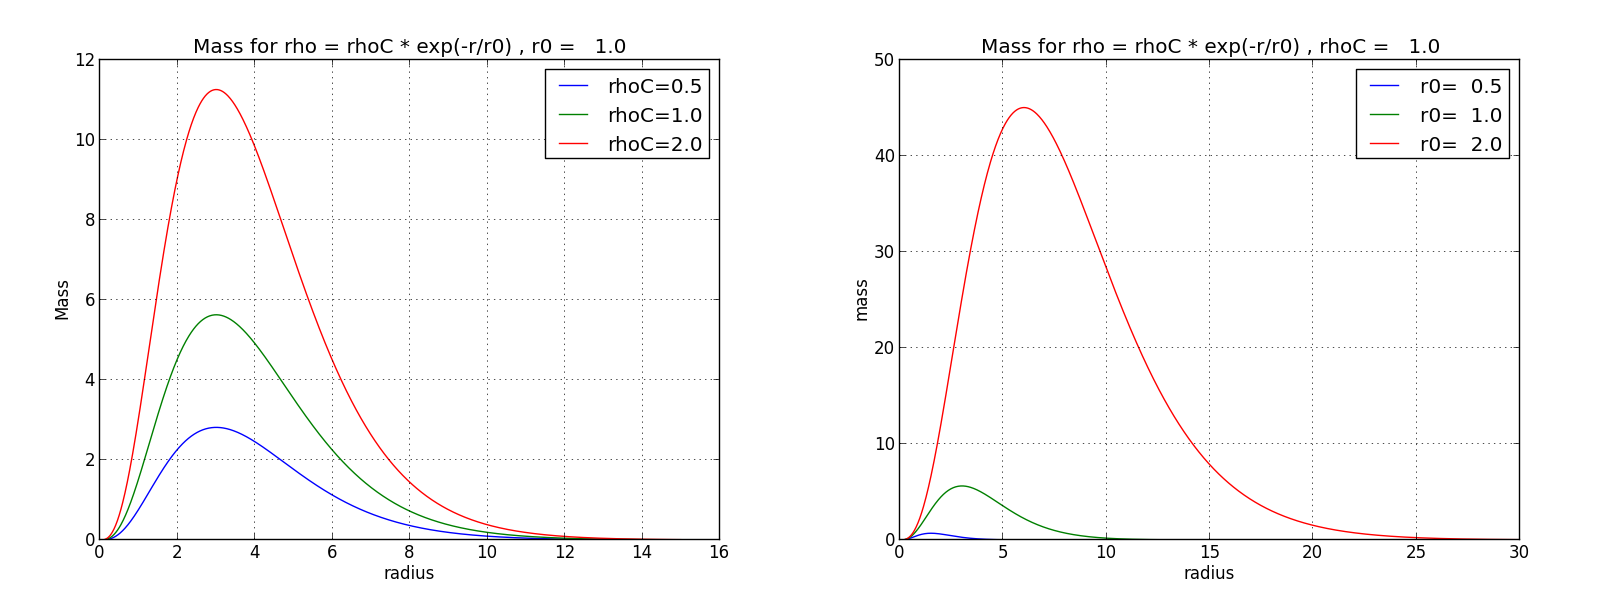
\includegraphics[scale=0.33]{massFinal.png}
 \caption{\emph{Masa}}
\end{figure}

\item

\begin{figure}[!ht]
 \centering
 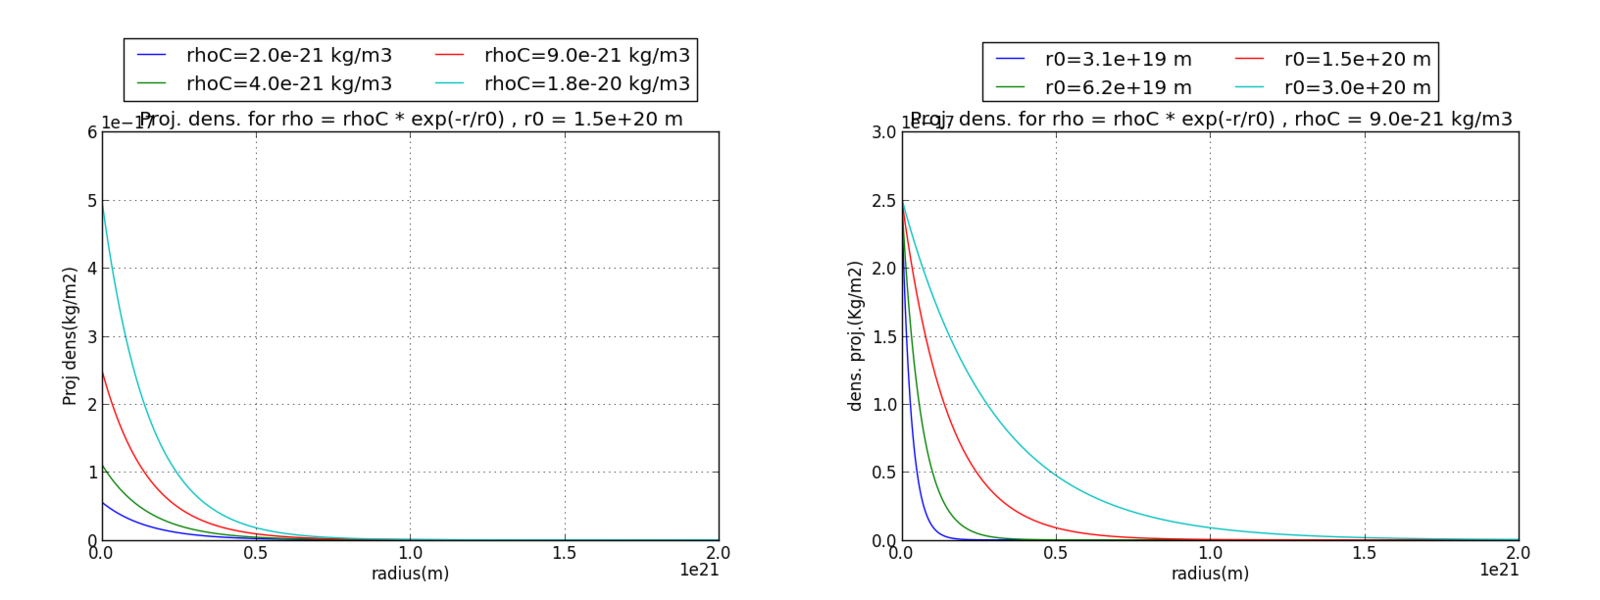
\includegraphics[scale=0.33]{dpFinal.png}
 \caption{\emph{Densidad proyectada}}
\end{figure}
\end{description}


\newpage


\begin{itemize}
	\item Hay otro programa python mas general que tiene como entrada la función de densidad (que puede tener parámetros que se pueden variar durante la ejecución a través de un slider) y calcula el potencial, velocidad circular, masa y distribución proyectada de masa según el caso general, pero tiene la posibilidad de representar el gráfico de las funciones calculadas de modo analítico
\item Para el potencial resolver la ecuación diferencial de segundo grado implica tener 2 constantes de integración, para la $V_c$ y masa hay solo una, variando la segunda constante en el caso del potencial y la única constante para la masa y velocidad y distribución proyectada solo hace una traslación a los gráficos de las funciones(sumando la constante), pero la forma queda igual así que solo tiene sentido tener en cuenta variar K1 en el caso del potencial 
\item Hay un slider con cual se puede cambiar el rango del radius desde 10**1 hasta 10**30
\item Se muestran los gráficos en el caso A = B = 1 ($\implies r_0= \rho_c =1$) y constantes de integración 0 para poder comprobarlos con los otros (donde hay 2 gráficos, el segundo está calculado con las fórmulas de la integración por partes: ver calc\_exp.py)

\begin{figure}[!ht]
 \centering
 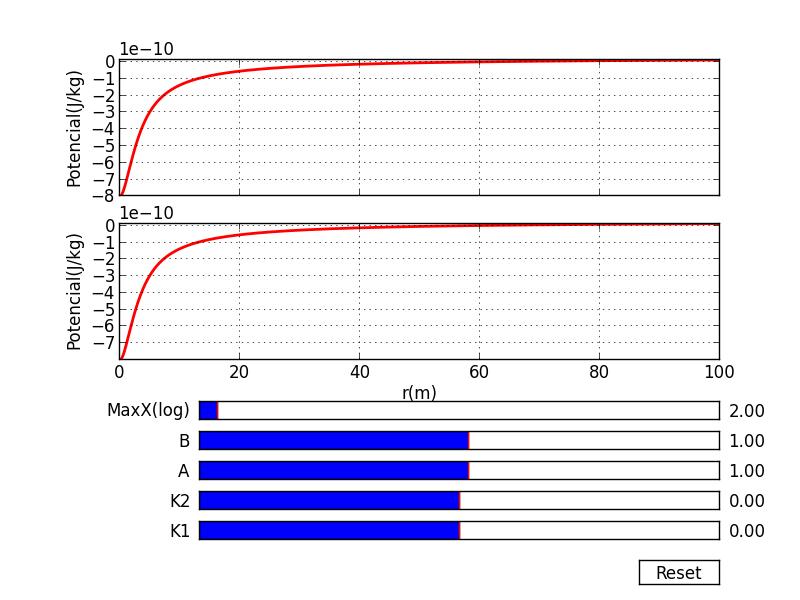
\includegraphics[scale=0.33]{pt_pot_A1_B1.png}
 \caption{\emph{Potencial}}
\end{figure}

\begin{figure}[!ht]
 \centering
 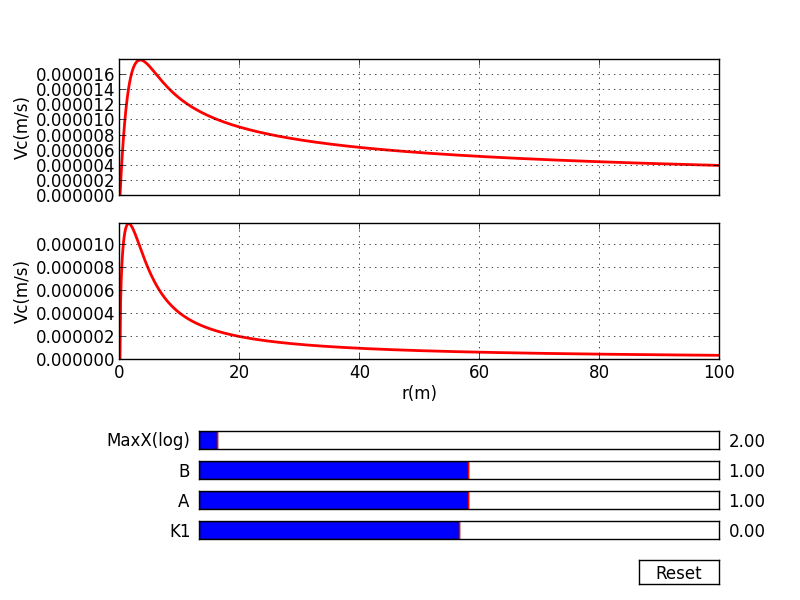
\includegraphics[scale=0.33]{pt_vc_A1_B1.png}
 \caption{\emph{Velocidad circular}}
\end{figure}

\begin{figure}[!ht]
 \centering
 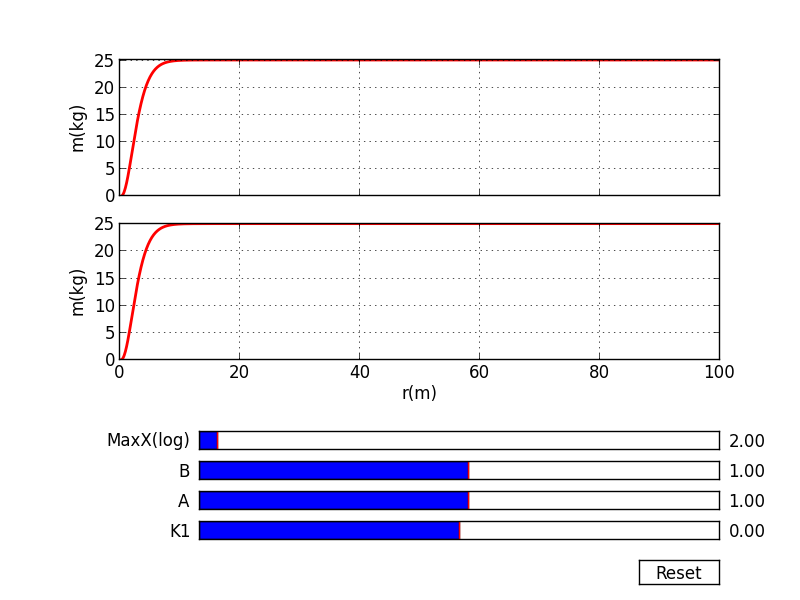
\includegraphics[scale=0.33]{pt_m_compAn.png}
 \caption{\emph{Masa}}
\end{figure}

\begin{figure}[!ht]
 \centering
 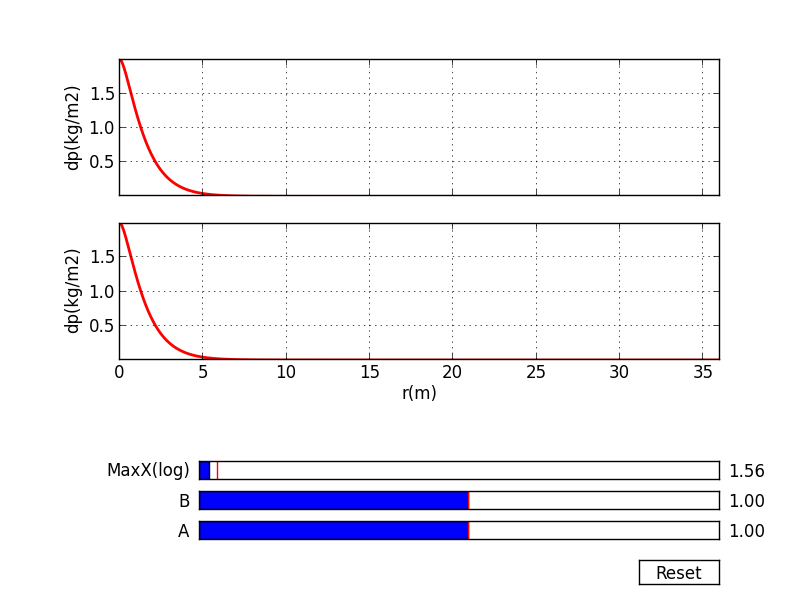
\includegraphics[scale=0.33]{pt_dp_compAn.png}
 \caption{\emph{Densidad proyectada}}
\end{figure}

\item Las figuras son las salidas para el caso  $ A > 0, B > 0 $ - el segundo gráfico es de la función calculada de forma analítica (con las fórmulas de la integración por partes, donde se añadieron las constantes de inetgarción)
\item La situación $ A < 0, B < 0 $ según se verá en los gráficos no tiene sentido físico. Además la función para determinar la distribución de densidad proyectada no es integrable

\end{itemize}
Potencial
\begin{itemize}
\item K1<0 hace que el término K1/r domine 

\item K1=0, el potencial crece desde 0 de forma asymptotica, la forma del gráfico no cambia variando A 
\begin{figure}[!h]
 \centering
 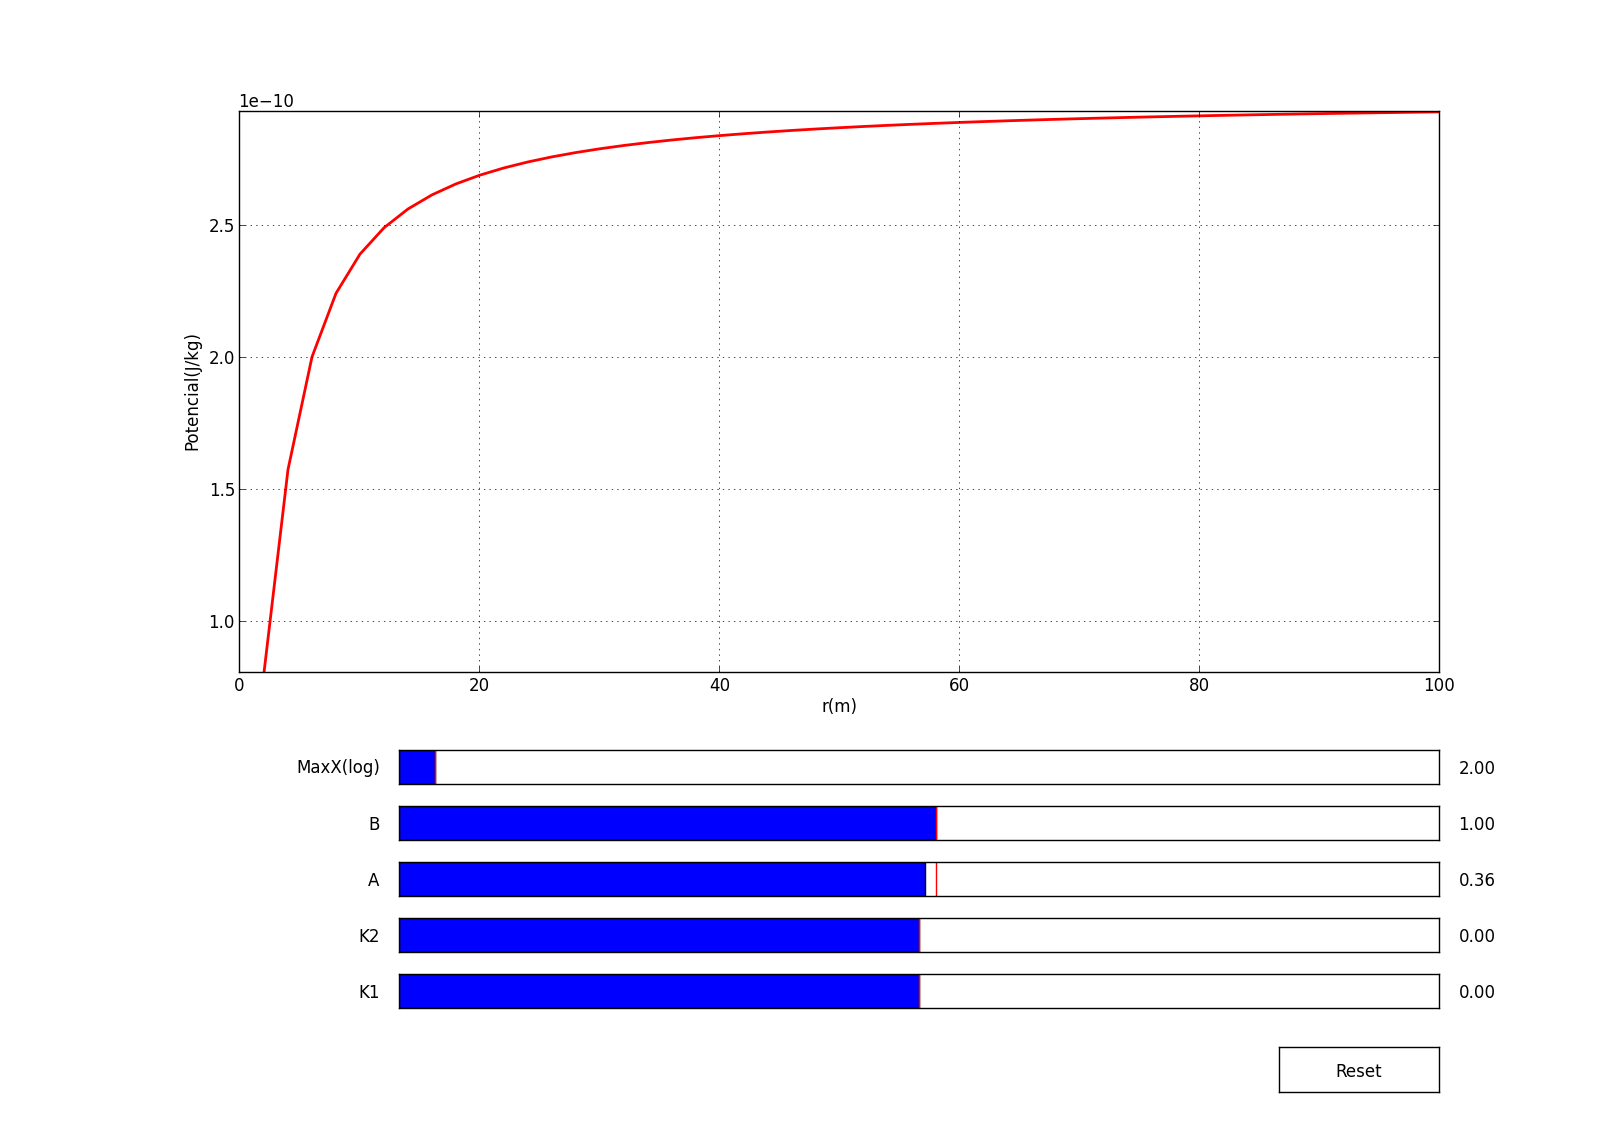
\includegraphics[scale=0.4]{p11.png}
 \caption{\emph{Potencial A mayor que 0, B = 1}}
 \label{Fig: 1}
\end{figure}

 
\end{itemize}



\begin{figure}[!h]
 \centering
 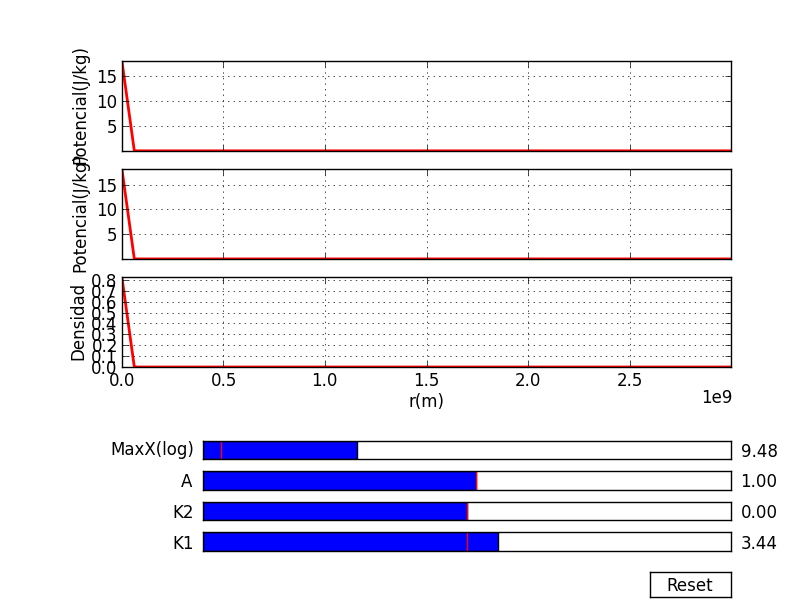
\includegraphics[scale=0.7]{potencial1.png}
 \caption{\emph{Potencial A = 1, rango del radio hasta 3*10**9}}
 \label{Fig: 1}
\end{figure}

\begin{figure}[!h]
 \centering
 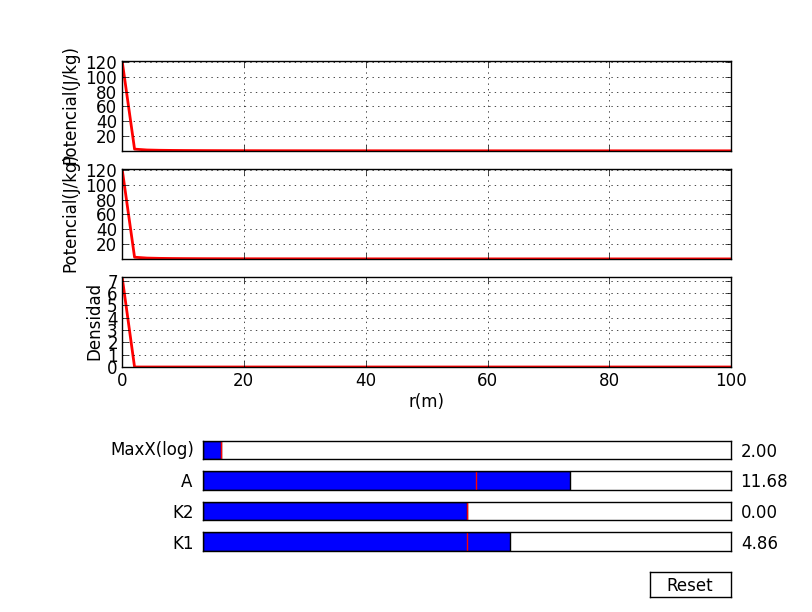
\includegraphics[scale=0.7]{potencial3.png}
 \caption{\emph{Potencial A mayor que 1}}
 \label{Fig: 3}
\end{figure}

\begin{figure}[!h]
 \centering
 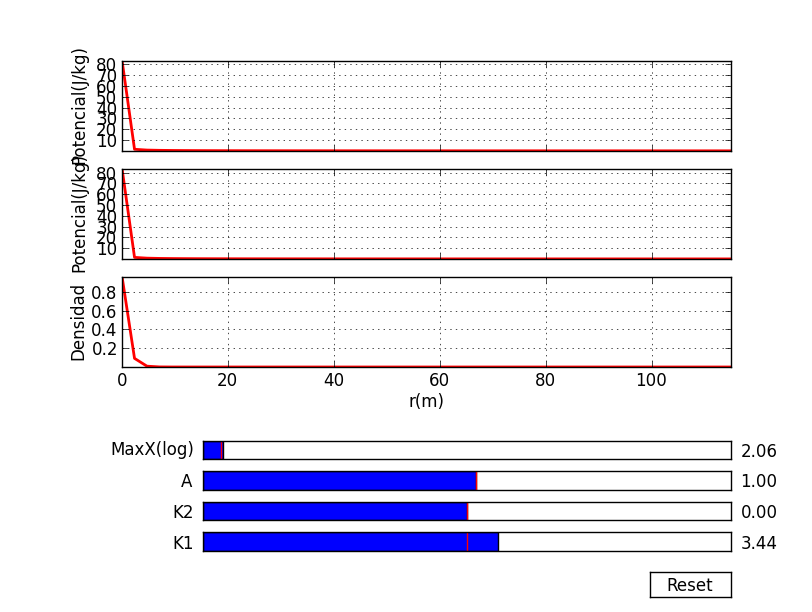
\includegraphics[scale=0.7]{potencial2.png}
 \caption{\emph{Potencial A = 1}}
 \label{Fig: 2}
\end{figure}


\begin{figure}[!h]
 \centering
 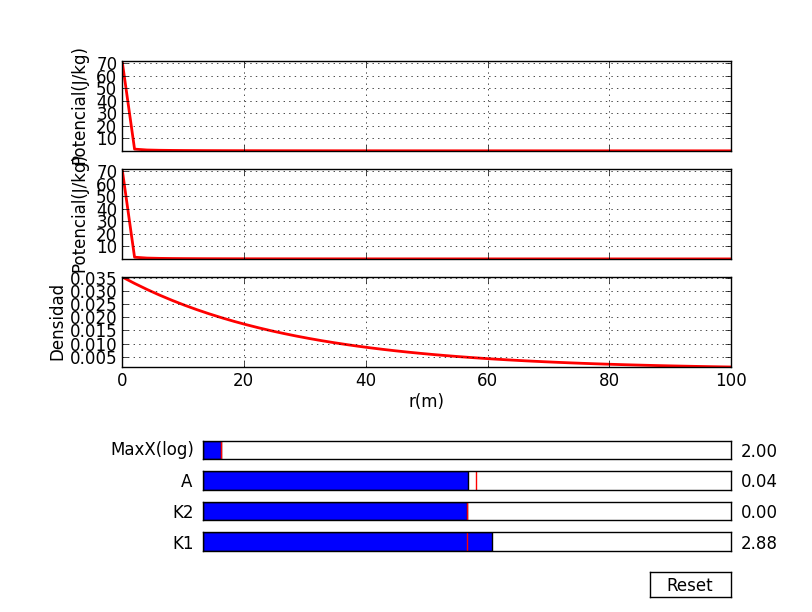
\includegraphics[scale=0.7]{potencial4.png}
 \caption{\emph{Potencial A in (0,1) }}
 \label{Fig: 1}
\end{figure}


\begin{figure}[!h]
 \centering
 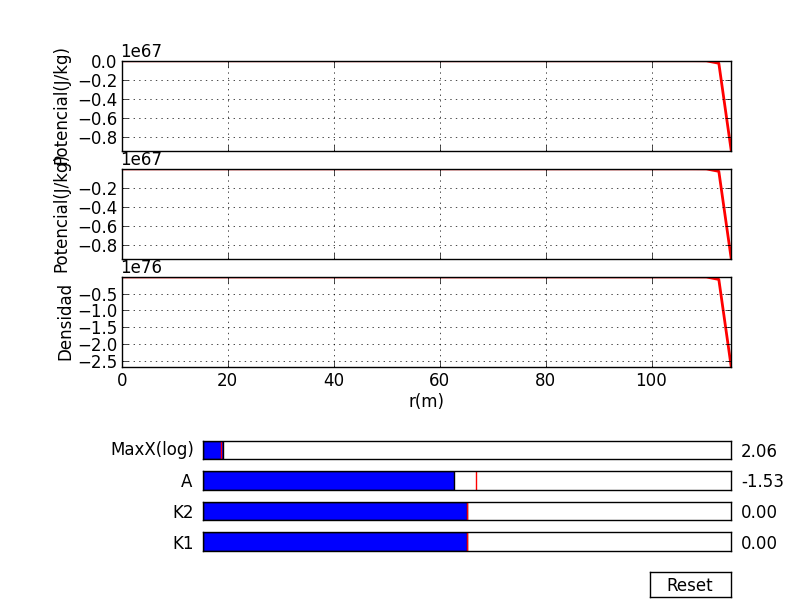
\includegraphics[scale=0.7]{potencial5.png}
 \caption{\emph{Potencial  A menor que 0}}
 \label{Fig: 1}
\end{figure}

\begin{figure}[!h]
 \centering
 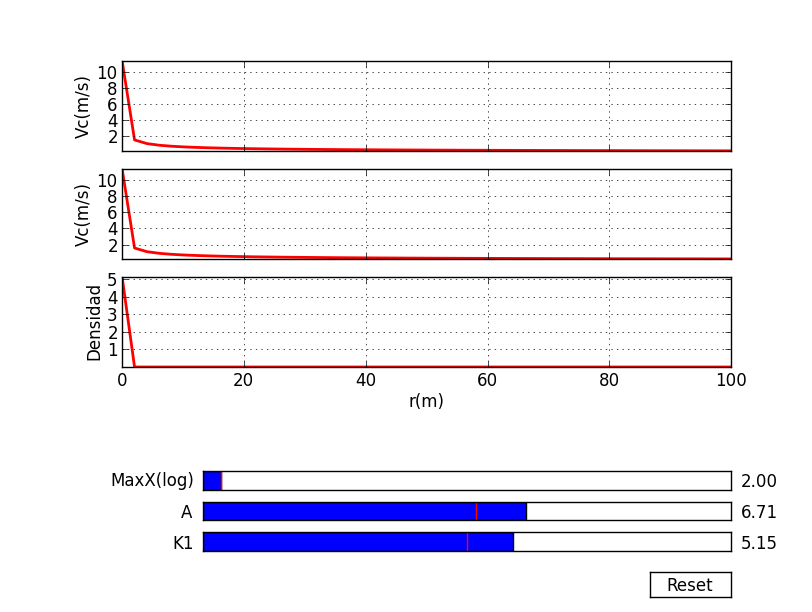
\includegraphics[scale=0.7]{velocity4.png}
 \caption{\emph{Vc A mayor que 1}}
 \label{Fig: 1}
\end{figure}

\begin{figure}[!h]
 \centering
 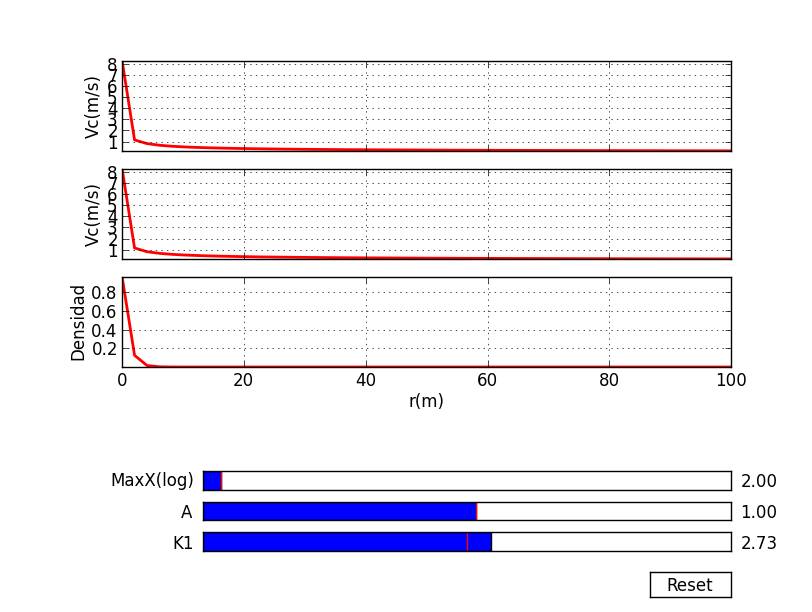
\includegraphics[scale=0.7]{velocity.png}
 \caption{\emph{Velocidad A = 1}}
 \label{Fig: 1}
\end{figure}

\begin{figure}[!h]
 \centering
 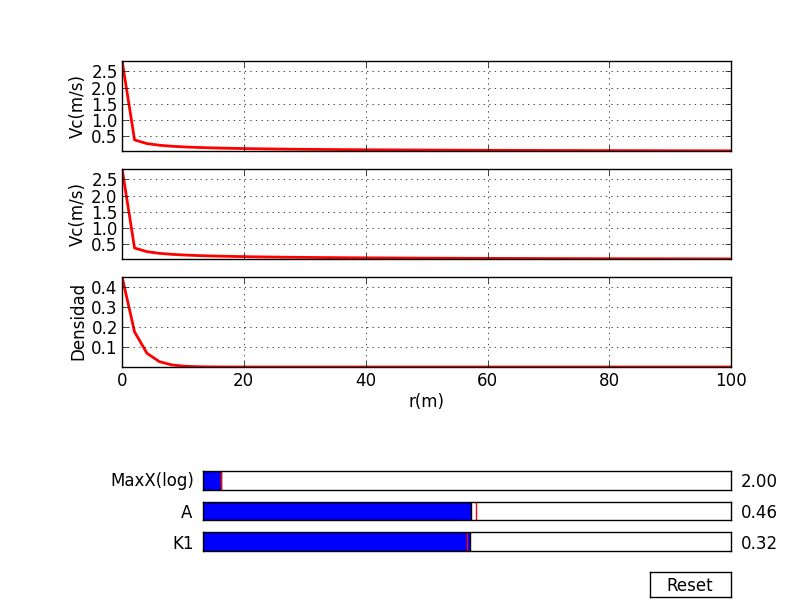
\includegraphics[scale=0.7]{velocity2.png}
 \caption{\emph{Vc A in (0,1) }}
 \label{Fig: 1}
\end{figure}

\begin{figure}[!h]
 \centering
 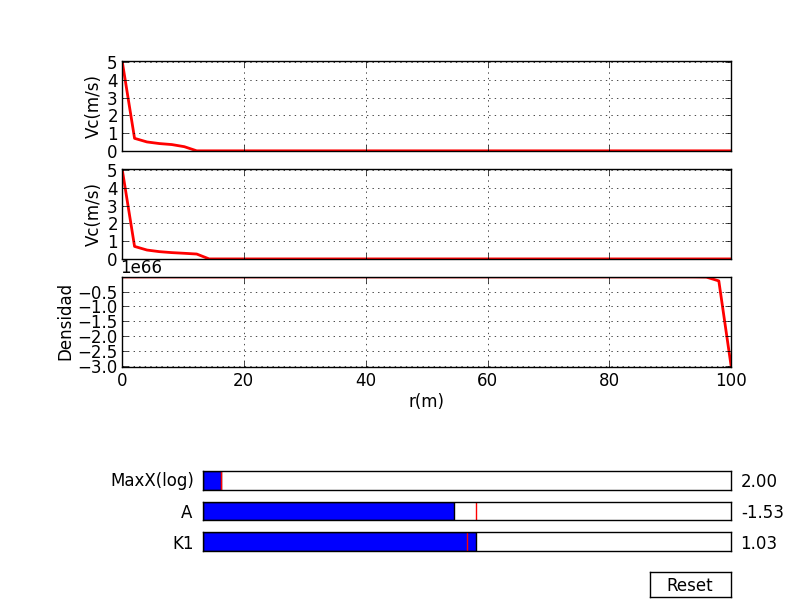
\includegraphics[scale=0.7]{velocity3.png}
 \caption{\emph{Velocidad circular A menor que 0}}
 \label{Fig: 1}
\end{figure}



\begin{figure}[!h]
 \centering
 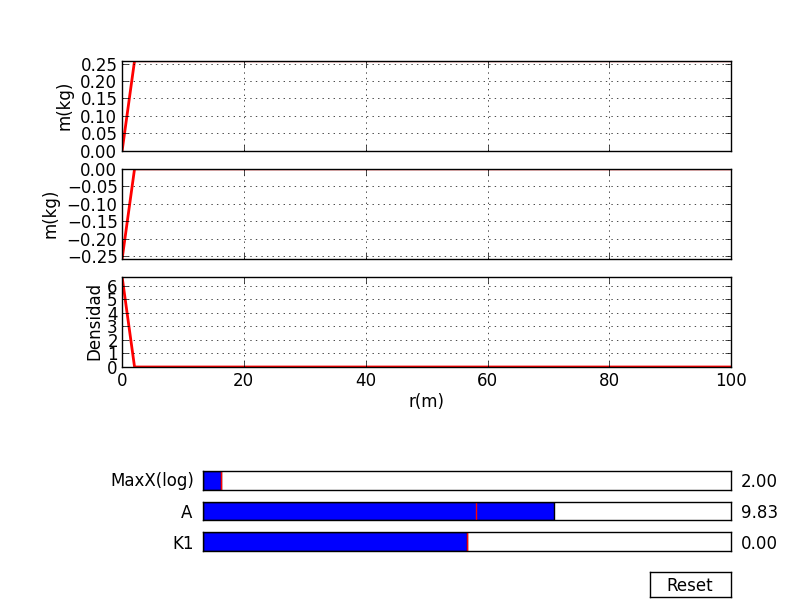
\includegraphics[scale=0.7]{masa4.png}
 \caption{\emph{Masa mayor que 1 }}
 \label{Fig: 1}
\end{figure}


\begin{figure}[!h]
 \centering
 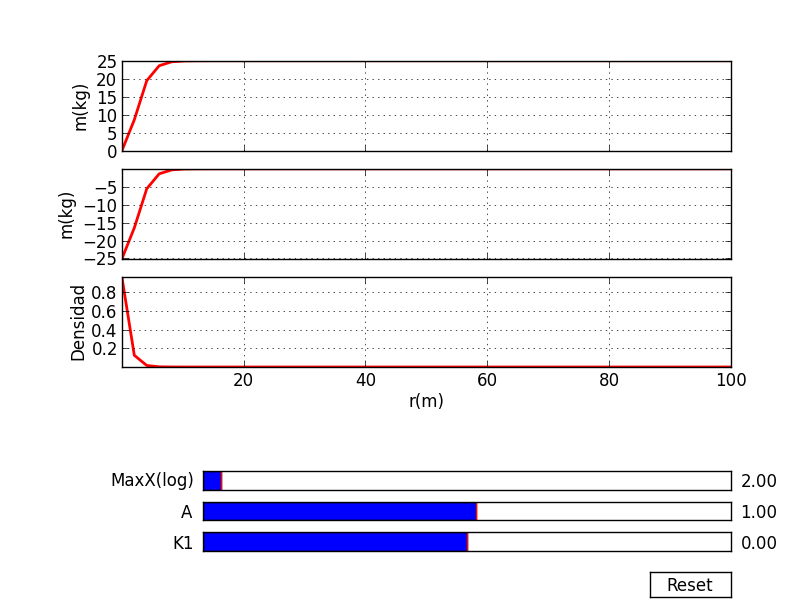
\includegraphics[scale=0.7]{masa1.png}
 \caption{\emph{Masa A = 1}}
 \label{Fig: 1}
\end{figure}

\begin{figure}[!h]
 \centering
 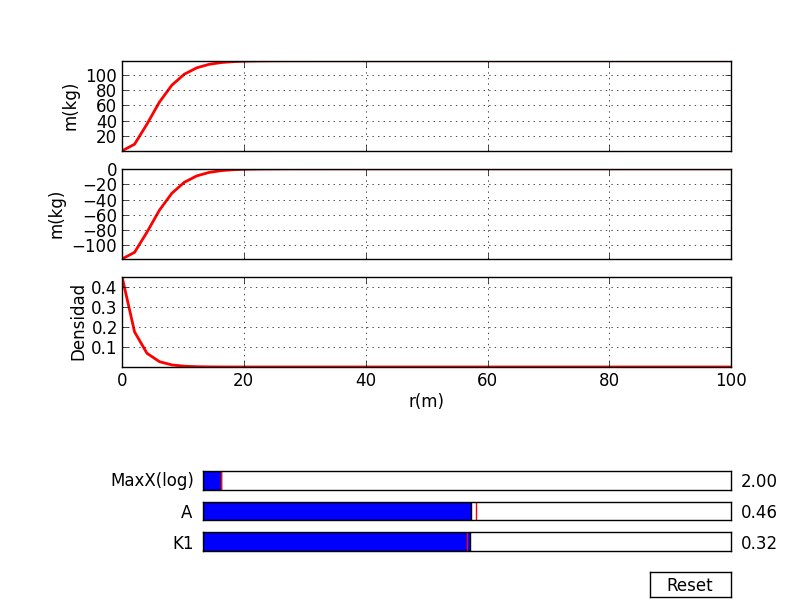
\includegraphics[scale=0.7]{masa2.png}
 \caption{\emph{Masa A in (0,1) }}
 \label{Fig: 1}
\end{figure}


\begin{figure}[!h]
 \centering
 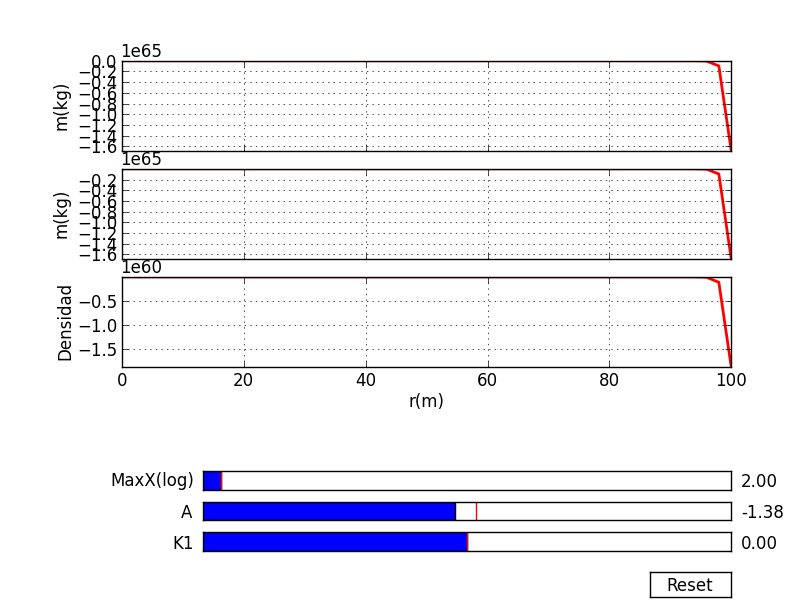
\includegraphics[scale=0.7]{masa3.png}
 \caption{\emph{Masa A menor que 0}}
 \label{Fig: 1}
\end{figure}



\begin{figure}[!h]
 \centering
 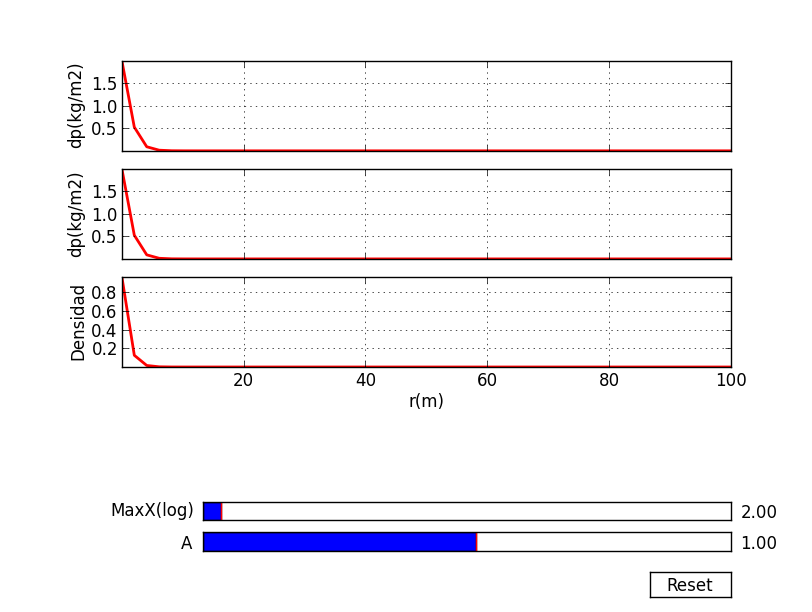
\includegraphics[scale=0.7]{dp1.png}
 \caption{\emph{Distribución proyectada A = 1}}
 \label{Fig: 1}
\end{figure}


\begin{figure}[!h]
 \centering
 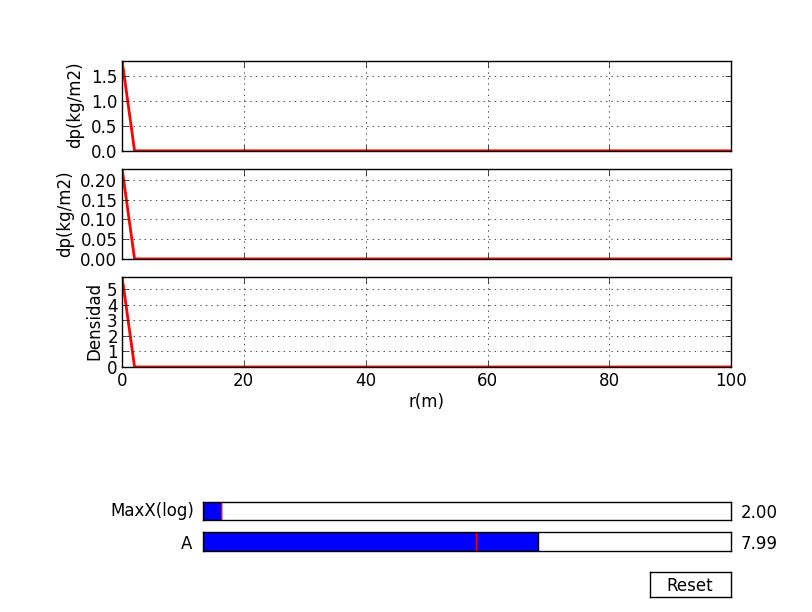
\includegraphics[scale=0.7]{dp2.png}
 \caption{\emph{Distribución proyectada A mayor que 1}}
 \label{Fig: 1}
\end{figure}

\begin{figure}[!h]
 \centering
 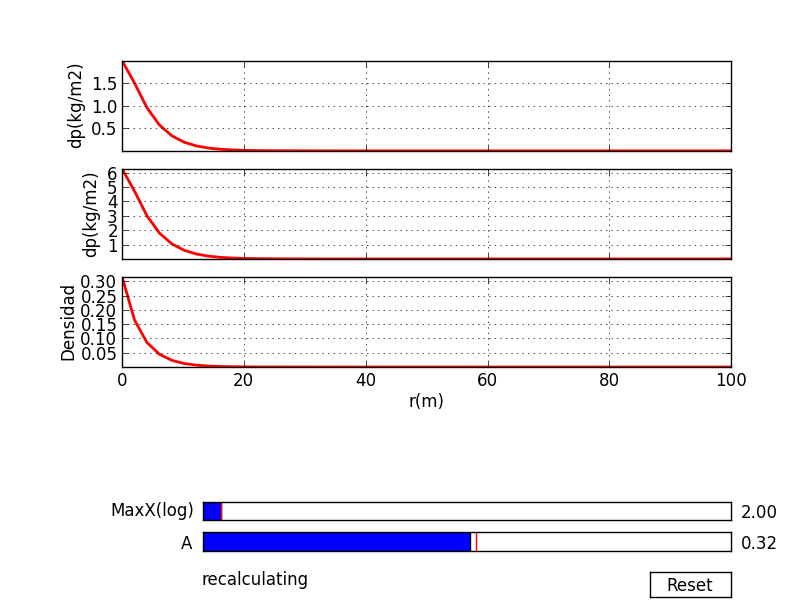
\includegraphics[scale=0.7]{dp3.png}
 \caption{\emph{Distribucion proyectada A in (0,1) }}
 \label{Fig: 1}
\end{figure}



\end{document}

